\documentclass[10pt,a4paper]{article}
\usepackage[a4paper,margin=2.1cm]{geometry}
\usepackage[T1]{fontenc}
\usepackage{lmodern,microtype}
\usepackage{amsmath,amssymb}
\usepackage{graphicx,booktabs,tabularx,multirow,array}
\usepackage{xcolor}
\usepackage{tikz}
\usetikzlibrary{arrows.meta,positioning,fit,backgrounds,calc,shapes.geometric}
\usepackage{algorithm,algpseudocode}
\usepackage{listings}
\usepackage{enumitem}
\usepackage{caption,subcaption}
\usepackage[colorlinks=true,linkcolor=teal!60!black,citecolor=teal!60!black,urlcolor=teal!60!black]{hyperref}
\usepackage{cleveref}

\definecolor{tanit}{HTML}{14B8A6}
\definecolor{ink}{HTML}{0F172A}
\definecolor{uca}{HTML}{8B5CF6}
\definecolor{ucb}{HTML}{06B6D4}
\definecolor{ucc}{HTML}{F43F5E}
\definecolor{ucd}{HTML}{F59E0B}
\definecolor{uce}{HTML}{10B981}
\lstset{basicstyle=\ttfamily\footnotesize,breaklines=true,frame=single,rulecolor=\color{black!20},
        backgroundcolor=\color{black!3},columns=fullflexible,keepspaces=true}
\newcommand{\tsf}{\textsc{Tanit Scenario Flywheel}}
\newcommand{\todo}[1]{\textcolor{red}{[#1]}}
\IfFileExists{results.tex}{\input{results.tex}}{%
  \newcommand{\ResultsUCone}{\todo{run make\_results.py}}%
  \newcommand{\ResultsUCthree}{\todo{run make\_results.py}}%
  \newcommand{\ResultsKPI}{\todo{run make\_results.py}}%
  \newcommand{\ResultsCosmos}{\todo{run make\_results.py}}%
  \newcommand{\ResultsUCtwo}{\todo{run make\_results.py}}%
  \newcommand{\ResultsUCfourfive}{\todo{run make\_results.py}}}

\title{\vspace{-1.2em}\textbf{\tsf}\\[0.3em]
\large An agentic, verifier-driven pipeline from scenario sources to multi-camera world-model data\\
and closed-loop evaluation on a single Jetson AGX Thor}
\author{TanitAD --- technical report}
\date{1 November 2026}

\begin{document}
\maketitle

\begin{abstract}
We present the \tsf, a production-oriented pipeline that turns five kinds of scenario sources --- free text,
single dash-cam videos, real-world AD incidents, sensor snippets with ground-truth ego motion and negative
fleet snippets --- into \emph{verified}, simulation-ready scenario descriptions (OpenDRIVE~1.8, OpenSCENARIO~1.3
XML and OpenSCENARIO DSL~2), renders them into consistent multi-camera and LiDAR data with NVIDIA Cosmos~3
world-scenario-map (WSM) conditioning, augments them along behavioural and appearance axes, and closes the
loop with an AD model under test --- without 3D Gaussian splatting. The central design decision is a typed
scenario intermediate representation (TSIR) that the local LLM (Qwen3.8-27B, NVFP4, on-device) emits under
grammar-constrained decoding, combined with a five-level \emph{hard} verifier ladder (schema, standards/XSD and
ASAM QC, lane-graph cross-check, simulation oracle, intent) whose findings are both the repair signal for the
agent and the reward for a Harness$^2$-style self-improving harness. Everything runs on one Jetson AGX Thor
(122\,GB unified memory). We report functional and speed KPIs for every stage.
\end{abstract}

\tableofcontents
\newpage

%=====================================================================================================
\section{Motivation and requirements}
Scenario-based testing of automated driving needs \emph{many} scenarios that are (i) relevant --- grounded
in real incidents, fleet data and expert intent, (ii) \emph{executable} --- standards-compliant and
simulator-ready, (iii) \emph{rich} --- with photorealistic multi-sensor data, and (iv) \emph{closed-loop
capable} --- so that the system under test can react. LLM-based generators produce plausible text but
fail silently on geometry, timing and semantics; neural renderers produce beautiful video but no ground
truth. The flywheel couples both through hard, executable verification.

\paragraph{Requirements (from the specification).}
\begin{enumerate}[nosep,leftmargin=1.4em]
\item Five use cases UC1--UC5 (\cref{tab:ucs}) feeding one shared flow.
\item Own 2D simulator that compiles, simulates and visualises OpenDRIVE/OSC1/OSC2 and extracts WSM/Cosmos data.
\item Own closed-loop simulator on Cosmos3-Nano-Sim-Auto that can host TanitAD models; test policies
      \emph{constant velocity} and \emph{accelerate--decelerate to standstill}; the TanitAD REFe SFT-4 policy under test.
\item Everything on the dedicated Jetson AGX Thor; operator UI on the engineer's PC.
\item Agentic steps on a local quantised Qwen3.8-27B; self-improving harness following Harness$^2$.
\item Camera/LiDAR rig following NVIDIA's PhysicalAI-AV standard; functional and speed KPIs.
\end{enumerate}

\begin{table}[h]\centering\small
\caption{Use cases. All converge on the TSIR and share verification, rendering, augmentation and closed loop.}\label{tab:ucs}
\begin{tabularx}{\linewidth}{@{}l l X@{}}\toprule
UC & Source & Flow \\\midrule
\textcolor{uca}{UC1} & text query & analyse $\to$ propose TSIR $\to$ verify/repair $\to$ document $\to$ simulate $\to$ WSM $\to$ Cosmos $\to$ augment $\to$ closed loop \\
\textcolor{ucb}{UC2} & dash-cam video & ViPE ego motion + intrinsics $\to$ road/agent lifting $\to$ TSIR $\to$ UC1 flow \\
\textcolor{ucc}{UC3} & AD incident (negative) & incident brief $\to$ counterfactual positive TSIR $\to$ IMDAD v2 twin $\to$ UC1 flow \\
\textcolor{ucd}{UC4} & sensor snippet + GT ego & log $\to$ TSIR (ego + tracked objects) $\to$ structured augmentation \\
\textcolor{uce}{UC5} & negative snippet & UC4 lifting $\to$ positive twin + variations $\to$ training data + closed loop \\\bottomrule
\end{tabularx}
\end{table}

%=====================================================================================================
\section{System architecture}
\Cref{fig:arch} shows the pipeline. Every source is lifted into the TSIR; deterministic compilers generate
all standard formats from it; the verifier ladder gates every artifact; the simulator produces ground-truth
tracks that drive both the 2D/3D viewer and the Cosmos WSM conditioning.

\begin{figure}[t]\centering
\resizebox{\linewidth}{!}{%
\begin{tikzpicture}[font=\sffamily\small,x=1cm,y=1cm,
  box/.style={draw=ink!45,rounded corners=3pt,fill=white,minimum height=9mm,inner sep=3pt,align=center,text width=#1},
  box/.default=24mm,
  core/.style={box=#1,fill=tanit!10,draw=tanit!70!black},core/.default=24mm,
  arr/.style={-{Stealth[length=2mm]},thick,draw=ink!55},
  fb/.style={-{Stealth[length=2mm]},thick,dashed}]
% sources
\foreach \i/\c/\t in {0/uca/{UC1 text query},1/ucb/{UC2 dash-cam video},2/ucc/{UC3 incident (IMDAD)},3/ucd/{UC4 sensor snippet},4/uce/{UC5 negative snippet}}
  \node[box=27mm,draw=\c,line width=0.9pt] (u\i) at (0,-1.15*\i) {\t};
\node[core=26mm,minimum height=30mm] (lift) at (4.2,-2.3) {\textbf{Lifter agents}\[2pt]\scriptsize Qwen3.8-27B NVFP4\\scriptsize xgrammar JSON\\scriptsize ViPE / log lifting};
\foreach \i in {0,...,4} \draw[arr] (u\i.east) -- ++(0.35,0) |- (lift.west);
\node[core=17mm,minimum height=14mm] (tsir) at (7.4,-2.3) {\textbf{TSIR}\\scriptsize typed IR};
\draw[arr] (lift) -- (tsir);
\node[box=25mm] (comp) at (10.4,-0.9) {compilers\\scriptsize .xodr\,·\,.xosc\,·\,.osc};
\node[box=25mm] (ver) at (10.4,-3.7) {verifier ladder\\scriptsize L0 schema \dots{} L3 oracle};
\draw[arr] (tsir.north) |- (comp.west);
\draw[arr] (tsir.south) |- (ver.west);
\draw[arr] (comp) -- (ver);
\node[core=24mm] (sim) at (13.6,-2.3) {\textbf{TanitSim}\\scriptsize ACC · signals · yield};
\draw[arr] (ver.east) -| node[pos=0.25,below,font=\scriptsize]{pass} (sim.south);
\node[box=25mm] (wsm) at (13.6,0.2) {WSM / RDS-HQ\\scriptsize 7 f-theta cams + LiDAR};
\node[core=25mm] (cos) at (17.0,0.2) {\textbf{Cosmos 3}\\scriptsize Transfer- / Sim-Auto};
\node[box=25mm] (aug) at (17.0,-2.3) {augmentation\\scriptsize Sobol + CEM + cells};
\node[box=25mm] (cl) at (13.6,-5.0) {closed loop\\scriptsize T0 kinematic · T1 neural};
\node[box=25mm] (pol) at (17.0,-5.0) {policy under test\\scriptsize TanitAD REFe SFT-4};
\draw[arr] (sim) -- (wsm); \draw[arr] (wsm) -- (cos);
\draw[arr] (sim) -- (aug);
\draw[arr] (sim) -- (cl);
\draw[arr] ([yshift=1.5mm]cl.east) -- ([yshift=1.5mm]pol.west);
\draw[arr] ([yshift=-1.5mm]pol.west) -- node[below,font=\scriptsize]{trajectory} ([yshift=-1.5mm]cl.east);
\draw[arr,dotted] (cos.east) -- ++(0.5,0) |- node[pos=0.25,right,font=\scriptsize,align=left]{camera frames\(sensor stage, T1)} (pol.east);
\node[box=30mm,fill=black!4] (h2) at (4.2,-5.4) {\textbf{Harness$^2$} library\\scriptsize prompts · skills · lessons · knobs};
\draw[fb,draw=ucc] (ver.south) -- ++(0,-0.45) -| node[pos=0.25,below,font=\scriptsize]{diagnostics $\rightarrow$ repair} ([xshift=6mm]lift.south);
\draw[fb,draw=tanit!70!black] (ver.south west) ++(0.3,0) |- node[pos=0.7,below,font=\scriptsize]{ladder score = reward} (h2.east);
\draw[fb,draw=tanit!70!black] (h2.north) -- (lift.south -| h2.north);
\end{tikzpicture}}
\caption{Flywheel architecture. Solid: data flow; dashed: verification diagnostics drive repair (red) and
harness self-improvement (teal); dotted: Cosmos as sensor stage of the neural closed-loop tier.}\label{fig:arch}
\end{figure}

\paragraph{Deployment.} One Jetson AGX Thor (JetPack 7.2.1, CUDA 13.2, 122\,GB unified memory, 14 Arm cores)
hosts: vLLM serving Qwen3.8-27B NVFP4 with an MTP speculative head (35\,\% memory budget), the Cosmos~3
models on demand, TanitSim, the verifier tools and a FastAPI service with a WebSocket event stream. The
React operator UI runs on the engineer's PC and talks only to that API.

%=====================================================================================================
\section{Tanit Scenario IR and compilers}
The TSIR is a small, typed, pydantic-validated JSON contract: environment; road (\texttt{linear} multi-segment
road of lines/arcs/clothoids, or a 3--5 arm \texttt{junction} with an optional fixed-time signal plan, or an
imported OpenDRIVE); actors with lane-relative initial positions, speeds and routes (turn sequences);
actions (speed change, lane change, follow, cut-in, stop at line, brake, crossing) with triggers (sim time,
signed distance to actor, TTC, distance to stop line, after-action chains); assertions (\cref{tab:assert});
and logical parameters (JSON pointers with ranges) for augmentation. Its JSON schema is handed to xgrammar,
so the LLM \emph{cannot} emit a syntactically invalid scenario --- it can only be wrong semantically, which
the ladder catches.

\paragraph{Compilers.} Deterministic and tested: (i) our own OpenDRIVE~1.8 writer --- junction arms start at
$R = r_\text{corner} + w_\text{half}$, connecting roads are normalised cubic-Hermite \texttt{paramPoly3}
curves with tangent length $k = c\,(1 + 0.27\,|\Delta h| / (\pi/2))$ (chord $c$), dynamic signals and
controllers; (ii) OpenSCENARIO~1.3 XML (storyboard with one maneuver group per actor, trigger and action
mapping, traffic-signal controller phases); (iii) OSC DSL~2 text; (iv) a standalone Python replay script.
We replaced a third-party junction generator after our L2 check found 8 of 32 lane links discontinuous by
up to 7\,m --- a concrete example of the verifier paying for itself.

\begin{table}[h]\centering\small
\caption{TSIR assertion kinds (simulation oracle, ladder level L3).}\label{tab:assert}
\begin{tabular}{@{}ll@{}}\toprule
assertion & meaning \\\midrule
\texttt{no\_collision} & no oriented-bounding-box overlap (SAT) between any actors\\
\texttt{min\_ttc\_above} & constant-velocity OBB time-to-collision of the ego stays above threshold\\
\texttt{ego\_lane\_change}, \texttt{ego\_turn} & intent: lane changes in a direction / turn type at a junction\\
\texttt{ego\_stops\_before\_line}, \texttt{red\_light\_respected} & regulatory behaviour at signals\\
\texttt{ego\_speed\_between}, \texttt{ego\_reaches\_s}, \texttt{max\_decel\_below} & kinematic envelope\\\bottomrule
\end{tabular}
\end{table}

%=====================================================================================================
\section{TanitSim: compile, simulate, visualise}
TanitSim parses OpenDRIVE~1.8 itself (line, arc, clothoid via Fresnel integrals, poly3, paramPoly3; lane
sections, widths, links and junction connections) into a sampled lane graph, so the simulator executes
\emph{exactly} what the compiler wrote. Longitudinal control uses the ACC model \cite{kesting2010acc}: the
IDM acceleration
\begin{equation}
a_\text{IDM} = a\Big[1-\Big(\tfrac{v}{v_0}\Big)^{4}-\Big(\tfrac{s^*(v,\Delta v)}{s}\Big)^2\Big],\quad
s^* = s_0 + vT + \tfrac{v\,\Delta v}{2\sqrt{ab}}
\end{equation}
blended with the constant-acceleration heuristic (CAH) so that cut-ins do not cause unrealistic emergency
braking ($c = 0.99$), followed by a jerk limiter ($6\,\text{m/s}^3$, $30\,\text{m/s}^3$ when entering braking).
Lane changes follow a quintic lateral profile; junction movements obey the signal plan (opposite-arm
groups, optional protected left phase) and permissive left turns yield to conflicting lanes (shapely
intersection of lane polygons). Collision is exact OBB overlap; TTC is computed by constant-velocity OBB
sweeping. An external ego (closed loop) is a kinematic bicycle tracked with pure pursuit.

\paragraph{Visualisation.} A cartographic renderer produces the showcase BEV videos (\cref{fig:bev}):
urban blocks or highway verges, sidewalks and curbs, lane markings (dashed/solid, double yellow, stop bars,
zebra crossings, turn arrows), speed-limit signs, signal heads with glow, category-specific vehicle sprites
with brake/indicator lights, TTC links, ego trail and a HUD (speed gauge, acceleration bar, event ticker,
minimap). Frames are rendered by a process pool (each worker builds the static map layer once).
The operator UI additionally offers an interactive 2D/3D (React Three Fiber) scene viewer.

\begin{figure}[t]\centering
\IfFileExists{figs/uc1_bev.png}{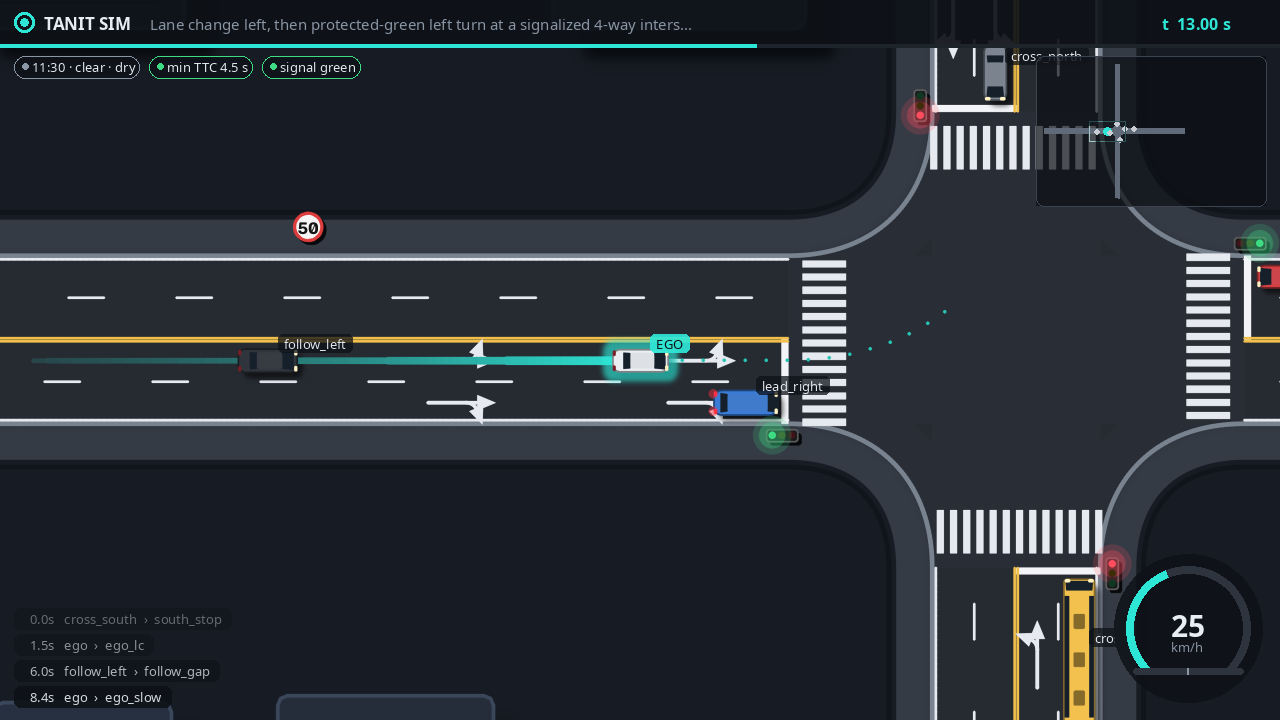
\includegraphics[width=0.49\linewidth]{figs/uc1_bev.png}}{\fbox{\parbox{0.47\linewidth}{\centering UC1 BEV frame}}}\hfill
\IfFileExists{figs/dci_bev.png}{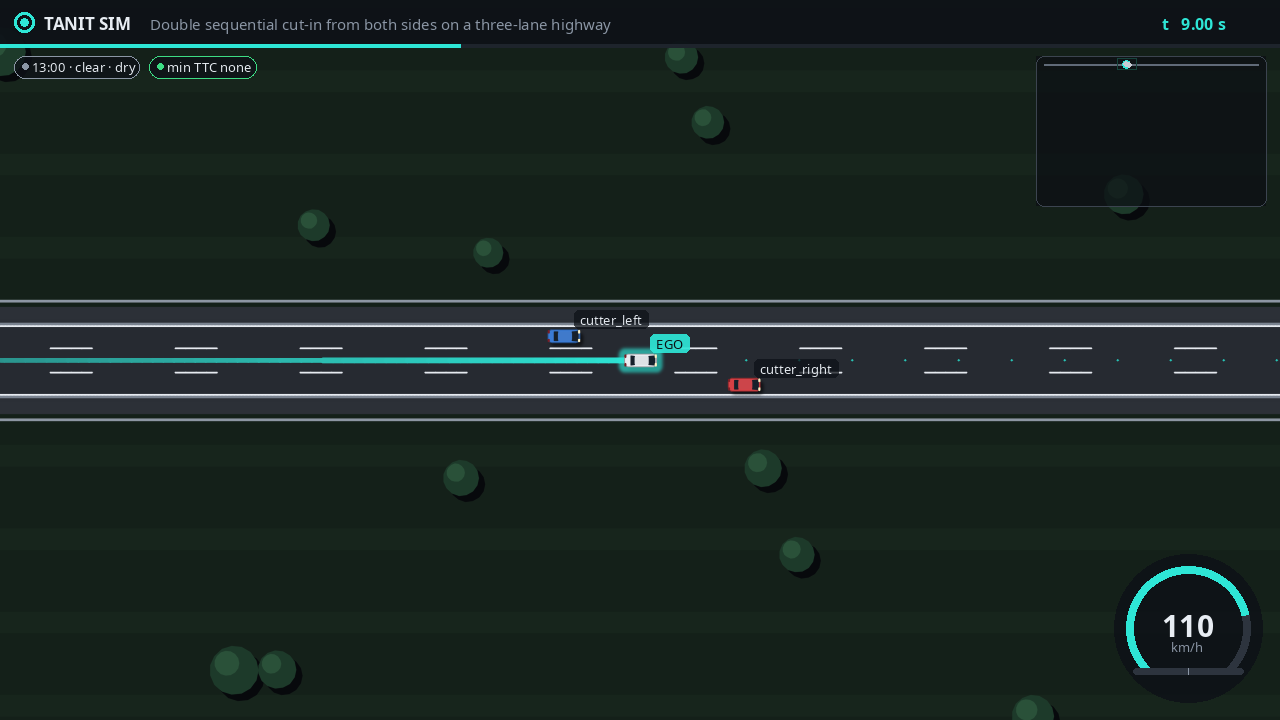
\includegraphics[width=0.49\linewidth]{figs/dci_bev.png}}{\fbox{\parbox{0.47\linewidth}{\centering double cut-in BEV frame}}}
\caption{TanitSim showcase renderer. Left: lane change left, then protected-green left turn at a signalized
4-way junction. Right: double sequential cut-in on a three-lane highway.}\label{fig:bev}
\end{figure}

%=====================================================================================================
\section{Verifier ladder and agentic lifting}
\begin{table}[h]\centering\small
\caption{Verifier ladder. The first failing level stops the ladder and returns structured diagnostics.}\label{tab:ladder}
\begin{tabularx}{\linewidth}{@{}l l X@{}}\toprule
level & check & implementation \\\midrule
L0 & schema & pydantic TSIR validation incl. referential integrity (actors, actions, triggers) \\
L1 & standards & compile; OpenDRIVE~1.8 XSD~1.1 (\texttt{xmlschema}), OpenSCENARIO~1.3 XSD (libxml2), ASAM QC OpenDRIVE bundle \\
L2 & cross-check & re-parse the written .xodr; lane-link continuity ($<0.1$\,m), junction movements, lane counts \\
L3 & oracle & simulate in TanitSim, evaluate all assertions; metrics (TTC, decel, jerk, turns, lane changes, red-light) \\
L4 & intent & LLM judge: does the simulated behaviour match the request? (planned) \\
L5 & plausibility & kinematic/statistical realism priors (planned) \\\bottomrule
\end{tabularx}
\end{table}

\paragraph{Lifter.} Four LLM roles share one model: \emph{analyst} (structured engineering analysis: actors,
assumptions with quantified values and sources, governing equations), \emph{proposer} (TSIR under xgrammar),
\emph{repairer} (receives the ladder diagnostics and simulation metrics) and \emph{documenter} (codeBeamer
description, derived functional requirements, variations). The final package follows the IMDAD scenario
structure; its \texttt{firstHypothesis} is the actual first attempt and \texttt{validationAndJudging} the
actual verifier findings, which makes every package a supervised training example for later SFT.

\paragraph{Decoding lessons.} Two failure modes of grammar-constrained decoding were found and fixed with the
KPI instrumentation: (1) with free JSON whitespace the model can enter an endless newline loop (visible as a
speculative-decoding acceptance length pinned at its maximum) --- fixed by a whitespace-free grammar;
(2) a repetition penalty, often recommended against loops, penalises JSON's own structural tokens and
derails long outputs (acceptance length collapses to 1.0) --- removed.

\ResultsUCone

%=====================================================================================================
\section{Self-improving harness (Harness$^2$ with hard verifiers)}
Following Harness$^2$ \cite{harness2}, model weights stay frozen and the \emph{harness} evolves: system prompt,
guardrails, tool guidance, skills (verified few-shot TSIRs), knobs (temperature, thinking, repair budget)
and an experience library of lessons with applicability keywords and evidence. Harness$^2$ is contrastive
and verifier-free; we add the ladder score as an objective reward:
\begin{equation}
\text{score} = \frac{\sum_{\ell=0}^{3} (\ell+1)\,\mathbb{1}[\text{L}\ell \text{ passed}]}{\sum_{\ell=0}^{3}(\ell+1)},
\end{equation}
so a Propose--Probe--Compose step (\cref{alg:h2}) adopts an edit only if matched probe runs show a score gain;
lessons stay \emph{candidate} until a human activates them in the UI.

\begin{algorithm}[h]\caption{Verifier-scored Propose--Probe--Compose}\label{alg:h2}\small
\begin{algorithmic}[1]
\State reference run on probe set $Q$ $\to$ failures $F$ with ladder diagnostics
\State \textbf{Propose}: invariant edit $e_I$ (prompt/guardrail) and domain edit $e_D$ (skill/lesson) from $F$
\State \textbf{Probe}: re-run $Q$ with $e_I$, $e_D$, $e_I\!+\!e_D$; score with the ladder (matched seeds)
\State \textbf{Compose}: adopt the best edit if $\Delta\text{score} > \epsilon$ and no regression; log revision + evidence
\end{algorithmic}
\end{algorithm}

%=====================================================================================================
\section{Augmentation}
Behavioural parameters (TSIR logical parameters) are explored with TanitSim as the cheap inner loop
(\cref{alg:aug}): a scrambled Sobol seed for coverage, cross-entropy-method iterations toward the
criticality boundary
\begin{equation}
c = \max\Big(\mathrm{clip}\big(\tfrac{3.0 - \mathrm{TTC}_\text{min}}{3.0-0.8}\big),\ \mathrm{clip}\big(\tfrac{a_\text{dec,max}-2}{4}\big)\Big),\qquad c=-1 \text{ on collision},
\end{equation}
and a novelty filter that keeps the most critical variant per coverage cell (LAMBDA-style \cite{lambda}).
Intent assertions (turns, lane changes, red light, progress) must still hold, so every variant is the
\emph{same} scenario. Appearance parameters (weather, time of day, surface) do not change the simulation;
they are crossed in at render time through the Cosmos prompt and WSM, multiplying every behavioural variant.

\begin{algorithm}[h]\caption{Criticality- and coverage-guided augmentation}\label{alg:aug}\small
\begin{algorithmic}[1]
\State $U \gets$ Sobol$(n_\text{seed}, d)$; evaluate each $u$ by simulation (metrics, $c$, intent)
\For{$k = 1..K$}
  \State elite $\gets$ top-25\,\% valid, non-colliding variants by $c$; fit $\mu,\sigma$ (floor 0.05)
  \State sample $n$ new $u \sim \mathcal{N}(\mu,\sigma)$ clipped to $[0,1]^d$; evaluate
\EndFor
\State keep $\arg\max_c$ per coverage cell; label \texttt{SYNTHETIC\_AUGMENTATION}, parent id
\end{algorithmic}
\end{algorithm}

\begin{figure}[h]\centering
\IfFileExists{figs/aug_coverage.png}{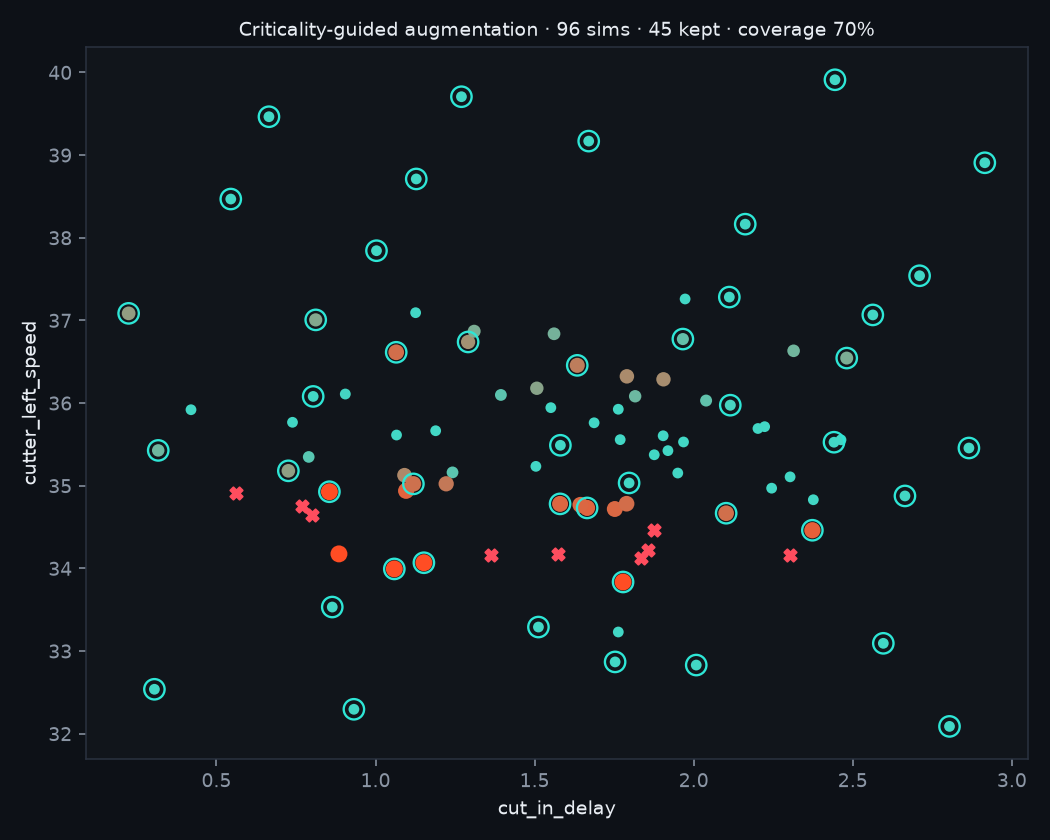
\includegraphics[width=0.62\linewidth]{figs/aug_coverage.png}}{}
\caption{Augmentation of the double cut-in: 96 simulations in 34\,s; the CEM concentrates samples at the
collision boundary (red crosses, cutter speed $\approx$34--35\,m/s); circles mark the 45 kept variants
(coverage 70\,\% of the $8\times8$ grid).}\label{fig:aug}
\end{figure}

%=====================================================================================================
\section{UC3: counterfactual positive twins from incidents}
For each NEGATIVE IMDAD~v2 incident the incident analyst writes a brief (failure mode, root cause,
normative behaviour with numbers, a replay request and a positive request with identical road, actors and
initial conditions). The Lifter turns the positive request into a verified TSIR; the twin is written as an
IMDAD~v2 record with \texttt{origin\_type = COUNTERFACTUAL\_POSITIVE}, \texttt{parent\_incident\_id}, the
verified package as \texttt{scenario\_specification} and simulated kinematics, and validated against
\texttt{incident\_schema\_v2} (including the referenced scenario schema). To our knowledge no prior work
generates verified positive twins from incident records \cite{sovar,crashagent}.

\ResultsUCthree

%=====================================================================================================
\section{WSM and Cosmos~3 rendering}
TanitSim logs are exported to the RDS-HQ layout (ego poses, 3D cuboid tracks, lanes, road boundaries, crosswalks,
signals) for the PhysicalAI-AV rig: seven f-theta cameras (front wide 120$^\circ$, front tele 30$^\circ$,
cross left/right 120$^\circ$, rear left/right 70$^\circ$, rear tele 30$^\circ$; 1920$\times$1080 at 30\,fps) and a
128-beam top LiDAR. The WSM renderer produces one control video per camera; Cosmos3-Nano-Transfer-Auto
generates photorealistic, cross-view-consistent video (and LiDAR) from these controls plus a text prompt
that carries the appearance parameters.

\ResultsCosmos

%=====================================================================================================
\section{Closed loop}
The same TanitSim world runs with a policy-driven ego. Tier T0 gives the policy privileged state (test
policies, planner debugging); tier T1 replaces the sensor stage with Cosmos3-Nano-Sim-Auto rendering of the
current world state, sim-time-decoupled (the world waits for the generator). Scoring follows the NAVSIM
EPDMS structure \cite{navsim}:
\begin{equation}
\text{EPDMS} = \text{NC}\cdot\text{DAC}\cdot\text{TLC}\cdot\frac{5\,\text{TTC} + 5\,\text{EP} + 2\,\text{C}}{12}.
\end{equation}
The policy under test is TanitAD REFe SFT-4 (ViT-L, 322M parameters, NAVSIM PDMS 88.25), which consumes four
NAVSIM pinhole cameras at 960$\times$512; an adapter reprojects the f-theta rig to these virtual pinholes.

\ResultsKPI

%=====================================================================================================
\section{UC2: dash-cam video to scenario}
NVIDIA ViPE \cite{vipe} estimates camera intrinsics, metric depth and camera poses from a single video.
The ego track (planar $x,y,\psi,v$ in a gravity-aligned frame) seeds the TSIR ego route and speed profile.

\ResultsUCtwo

%=====================================================================================================
\section{UC4/UC5: sensor snippets with ground-truth ego motion}
Snippets come from NVIDIA PhysicalAI-AV (internal validation only): ground-truth egomotion ($\approx$100\,Hz) and
auto-labelled 3D obstacle tracks ($\approx$10\,Hz). Clips are selected through the dataset's out-of-distribution
reasoning annotations (event cluster, timestamp, cause). \emph{Lifting} is deterministic: the ego path, low-passed
over 25\,m so that lane changes and nudges remain lateral offsets, becomes the road reference; tracks are mapped to
Frenet coordinates; lane topology follows from the lateral distribution of same-direction and oncoming traffic;
speed profiles are segmented (Douglas--Peucker) into \texttt{speed\_change}, lane-index changes into
\texttt{lane\_change}, sustained in-lane excursions into the new \texttt{lane\_offset} action (OpenSCENARIO
\texttt{AbsoluteLaneOffsetAction}); vehicles first seen later are back-extrapolated to $t_0$. The lifted scenario
is re-simulated and compared with the log (\emph{fidelity}); collisions in the re-simulation reveal lifting errors and
are removed by a deterministic de-conflict pass. UC5 treats the lifted snippet as the NEGATIVE: the twin editor (LLM)
writes only an \emph{ego plan} that is spliced into a copy of the negative, so every other road user keeps its logged
behaviour by construction; the positive must pass relative criteria (no collision, peak deceleration below
$0.75\times$ the negative's, TTC $\geq$ 2\,s).

\ResultsUCfourfive

%=====================================================================================================
\section{Data governance}
Code, documentation, this report and the IMDAD schemas are public. Never published: credentials, proprietary
fleet recordings and anything derived from them (processed on the Thor only; aggregate metrics only), dataset
frames under non-redistribution licences (PhysicalAI-AV: internal validation only), and incident records.

\section{Conclusion and next steps}
\todo{fill after results}

\begin{thebibliography}{99}\small
\bibitem{harness2} C.-Y.~Lee, T.~Pfister et al. Harness$^2$: Recursive agent harnessing for an open world. arXiv:2610.14224, 2026.
\bibitem{kesting2010acc} A.~Kesting, M.~Treiber, D.~Helbing. Enhanced intelligent driver model to access the impact of driving strategies on traffic capacity. \emph{Phil. Trans. R. Soc. A}, 2010.
\bibitem{lambda} LAMBDA: coverage-guided scenario generation. arXiv:2412.00517.
\bibitem{navsim} D.~Dauner et al. NAVSIM: data-driven non-reactive autonomous vehicle simulation and benchmarking; EPDMS metric definition, NAVSIM v2. 2024--2025.
\bibitem{sovar} SoVAR: crash reports to simulation via LLM + constraint solving. arXiv:2409.08081.
\bibitem{crashagent} CrashAgent: multi-agent crash reconstruction and counterfactuals. arXiv:2505.18341.
\bibitem{chatscene} ChatScene: knowledge-enabled safety-critical scenario generation. arXiv:2405.14062.
\bibitem{text2scenario} Text2Scenario: text-driven OpenSCENARIO generation. arXiv:2503.02911.
\bibitem{gepa} GEPA: reflective prompt evolution. arXiv:2507.19457.
\bibitem{ace} ACE: agentic context engineering with evolving playbooks. arXiv:2510.04618.
\bibitem{vipe} NVIDIA. ViPE: video pose engine for geometric 3D perception. github.com/nv-tlabs/vipe, 2025.
\bibitem{cosmos} NVIDIA. Cosmos~3 world foundation models (Nano Transfer-Auto, Sim-Auto). 2026.
\bibitem{asamqc} ASAM e.V. Quality checker framework and OpenDRIVE checker bundle. 2025.
\end{thebibliography}
\end{document}
